
\Appendix{Inference of Conditional Random Field Model}
\label{apdx:crf}
The first model comes to mind.

\section{Potential Function}
Each grid is a node, and its crime rate $y_i$ is the hidden variable that we want to estimate. Two kinds of fixed parameters are observed for each grid $g_i$. The first one is the demographic features $\x_i$. The second is the interactions among grids, such as social flow and geospatial distance, denoted by $\f{ij}$.

We use Conditional Random Field (CRF) shown in Figure~\ref{fig:crf} to model the dependency of nodal features. The learning goal is to estimate the conditional probability of $y$ given $\x$ and $\f$

\begin{equation}
	P(y |  \x, \f) 
\end{equation}


\begin{figure}[hb]
	\centering
	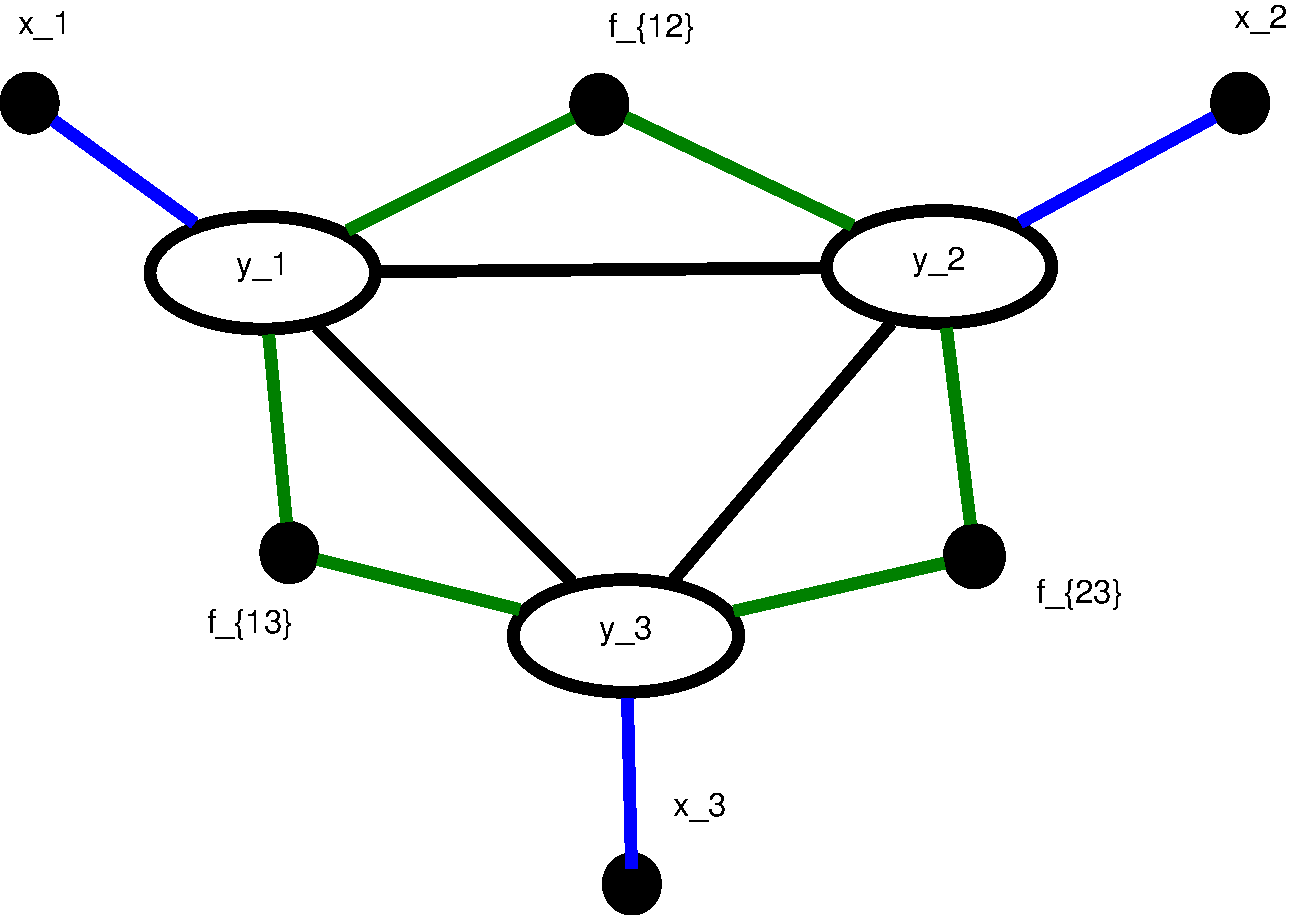
\includegraphics[width=0.5\textwidth]{fig/CRF-fig.pdf}
	\caption{The CRF model of the crime rate $y_i$ for each grid $g_i$.}
	\label{fig:crf}
\end{figure}



In the CRF model, we factorize the probability distribution of $y$ to a series of potential functions $\psi$ on the clique. 
\begin{equation}
	P(Y) = \frac{1}{Z} \prod_{ c \in C} \psi(c)
\end{equation}

Use $C_1$ to denote the set of cliques of size 1 with the form $\langle y_i \rangle$, and $C_2$ to denote size-2 clique. We define the potential function as follows:

\begin{align}
	\psi_{C_1} = &exp( - |y_i - \demow^T \cdot \x_i| )  \forall i \in [1, n], {g_i} \in C_1, \\
	\psi_{C_2} = & exp( - |y_i - y_j - \w^T \cdot \f_{i,j}| )  \forall i,j \in [1, n], {g_i, g_j} \in C_2, 
\end{align}
where $\demow$ and $\w$ are all positive coefficients.

The distribution of $Y$ is given by 
\begin{equation}
	P(Y) =  \frac{1}{Z} \left[ \prod_{i=1}^n \psi_{C_1}(y_i) \times \prod_{i=1}^n \prod_{j=i}^n \psi_{C_2}(y_i, y_j) \right]
\end{equation}
\begin{multline}
	P(Y) =  \frac{1}{Z} exp  \left( - \sum_{i=1}^n |y_i - \demow^T \cdot \x_i| \right. \\
          \left. - \sum_{i=1}^n\sum_{j=i}^n |y_i - y_j - \w^T \cdot \f_{i,j}| \right)
	\label{eq:PY}
\end{multline}


A large value of  potential function $\psi$ implies the high probability of $P(Y)$. The goal is to find a set of $Y$ maximizing $P(Y)$. 


\section{Inference}


\subsection{Estimate CRF Parameters}
\label{sec:estim}


We solve the Equation~(\ref{eq:PY}) by minimizing the negative log-likelihood function
\begin{multline}
\min_{\demow, \w} -\log P(Y|\demow, \w) = \min_{\demow, \w} \left[ \log Z + \sum_{i=1}^n |y_i - \demow^T \cdot \x_i| \right. \\
\left.  + \sum_{i=1}^n\sum_{j=i}^n |y_i - y_j - \w^T \cdot \f_{i,j}| \right]
\end{multline}

Use matrix form
\[
\min_{\demow, \w} ||X \demow - \y||_1 + ||F \cdot \w - \yp||_1,
\]
where $X$ is demographics matrix with $n$ rows, $\y$ is the $n$-dimension crime rate vector, $F$ is the pairwise features matrix with $(n^2+n)/2$  rows, and $\yp$ is the $(n^2+n)/2$-dimension pairwise crime rate difference vector $\{y_i- y_j\}$.

We can minimize separably.



\textbf{Minimize $\demow$}

\[ \min_{\demow} ||X \demow - \y||_1 \]

Take $X\demow - \y = \z$, and use ADMM.
\begin{multline}
 \min_{\z, \demow}  ||\z||_1 + \rho/2 ||\z - X\demow + \y||_2^2,\\
   s.t.\quad  \z - X\demow + \y = 0 
\end{multline}

\begin{multline}
L(\vec{\theta_1}, \z, \demow) = \max_{\vec\theta_1} \min_{\z, \demow} ||\z||_1 + \\
\rho/2 ||\z - X\demow + \y||_2^2  + \vec{\theta_1}( \z - X\demow + \y ) 
\end{multline}

\textbf{$\demow$ update}

\[ \demow^{k+1} \gets \argmin_{\demow}  \rho/2 ||\z^{k+1} - X\demow + \y + \vec{\theta_1}^{k+1}||_2^2 \]
Take derivative we have
\[ \frac{\partial}{\partial \demow} = \rho X^T(X\demow - \z^{k+1} - \y - \vec\theta_1^{k+1} ) \]
Make it $0$, $\demow^{k+1} = (X^TX)^{-1} X^T(\z^{k+1} + \y + \vec\theta_1^{k+1})$.

\textbf{$\z$ update}

\[ \z^{k+1} \gets \argmin_{\z}  ||\z||_1 + \rho/2 ||\z - X\demow^{k+1} + \y + \vec{\theta_1}^{k+1}||_2^2 \]
So, $\z^{k+1} = S_{1/\rho}(X\demow^{k+1} - \y - \vec\theta_1^{k+1})$.

\textbf{$\vec\theta_1$ update}

\[ \vec\theta_1^{k+1} = \vec\theta_1^{k} + \z^{k+1} - X\demow^{k+1} + \y \]



\textbf{Minimize $\w$}

\[ \min_{\w} ||F \cdot \w - \yp||_1 \]
It has exactly the same form as previously. Therefore,
\begin{multline}
L(\vec{\theta_2}, \z', \w) = \max_{\vec\theta_2} \min_{\z', \w}  ||\z'||_1 + \\
\rho/2 ||\z' - F\w + \yp||_2^2 + \vec{\theta_2}( \z' - F\w + \yp ) 
\end{multline}

\textbf{$\w$ update}
\[ \w^{k+1} = (F^TF)^{-1} F^T(\z^{'k+1} + \yp + \vec\theta_2^{k+1}) \]

\textbf{$\z'$ update}
\[ \z^{'k+1} = S_{1/\rho}(F\w^{k+1} - \yp - \vec\theta_2^{k+1}) \]

\textbf{$\vec\theta_1$ update}
\[ \vec\theta_2^{k+1} = \vec\theta_2^{k} + \z^{'k+1} - F\w^{k+1} + \yp \]



\subsection{Infer New $y_i$}

To infer new $y_i$, we want to maximize the following probability
\[ P(y_i | \x_i, F, \y, \demow, \w), \]
where $\demow$ and $\w$ are estimated using previous section, $\y$ denote the crime rates of other observed geographical units, and $F$ is the pairwise feature matrix.

Take negative log of the probability, we have 

\begin{align}
\min_{y_i} &  \left[ \log Z +  |y_i - \demow^T \cdot \x_i| + \sum_{j \neq i}^n |y_i - y_j - \w^T \cdot \f_{i,j}| \right] \nonumber \\
\min_{y_i} & \left[ |y_i - \demow^T \cdot \x_i| + \sum_{j \neq i}^n |y_i - y_j - \w^T \cdot \f_{i,j}| \right] 
\label{eq:inference}
\end{align}

In Equation~\ref{eq:inference}, we have $n+1$ $\ell_1$-norm terms, which have exactly the same form $|y_i - b_j|$. The objective becomes
\begin{equation}
  \min_{y_i} \sum_j^n |y_i - b_j|,
\label{eq:infy}
\end{equation}
where $b_1 = \demow^T \cdot \x_i$ and $b_j = y_{j-1} + \w^T\cdot \f_{i,j-1}$ for $j > 1$.

Notice that the optimal solution must take value on $\{b_j\}$. We solve this by sorting all the $b_j$ and then calculate the result segment by segment.